\documentclass[10pt,a4j]{jarticle}
%\usepackage{graphicx,wrapfig}
\usepackage{graphicx}
\setlength{\topmargin}{-1.5cm}
%\setlength{\textwidth}{16.5cm}
\setlength{\textheight}{25.2cm}
\newlength{\minitwocolumn}
\setlength{\minitwocolumn}{0.5\textwidth}
\addtolength{\minitwocolumn}{-\columnsep}
%\addtolength{\baselineskip}{-0.1\baselineskip}
%
\def\Mmaru#1{{\ooalign{\hfil#1\/\hfil\crcr
\raise.167ex\hbox{\mathhexbox 20D}}}}
%
\begin{document}
\newcommand{\fat}[1]{\mbox{\boldmath $#1$}}
\newcommand{\D}{\partial}
\newcommand{\w}{\omega}
\newcommand{\ga}{\alpha}
\newcommand{\gb}{\beta}
\newcommand{\gx}{\xi}
\newcommand{\gz}{\zeta}
\newcommand{\vhat}[1]{\hat{\fat{#1}}}
\newcommand{\spc}{\vspace{0.7\baselineskip}}
\newcommand{\halfspc}{\vspace{0.3\baselineskip}}
\bibliographystyle{unsrt}
%\pagestyle{empty}
\newcommand{\twofig}[2]
 {
   \begin{figure}
     \begin{minipage}[t]{\minitwocolumn}
         \begin{center}   #1
         \end{center}
     \end{minipage}
         \hspace{\columnsep}
     \begin{minipage}[t]{\minitwocolumn}
         \begin{center} #2
         \end{center}
     \end{minipage}
   \end{figure}
 }
%%%%%%%%%%%%%%%%%%%%%%%%%%%%%%%%%
%\vspace*{\baselineskip}
\begin{flushright}
構造力学II\\ 2020/04/20
\end{flushright}
\begin{center}
	{\LARGE \bf 講義ノート1} \\
\end{center}
%%%%%%%%%%%%%%%%%%%%%%%%%%%%%%%%%%%%%%%%%%%%%%%%%%%%%%%%%%%%%%%%
\section{1次元軸力問題}
\subsection{強形式(復習)}
\subsubsection{支配方程式}
1次元軸力問題の支配方程式は
\begin{equation}
	\frac{d}{dx}\left(EA \frac{du}{dx}\right) + p =0, \ \ \left(x\in (0,l)\right)
	\label{eqn:gveq}
\end{equation}
で与えられる.ここに,$u$は軸変位を,$E$はヤング率,$A$は部材の断面積を表す.
また,$p(x)$は部材軸方向に働く分布力で,単位長さあたりの力の次元を持つ量で,
$x$は部材長手方向にとった座標である.
式(\ref{eqn:gveq})は, 軸力$N$に関する釣り合い条件:
\begin{equation}
	\frac{dN}{dx}+p=0, \ \ \left(x\in (0,l)\right)
	\label{eqn:equiv_N}
\end{equation}
と,フックの法則:
\begin{equation}
	\sigma=E\varepsilon
	\label{eqn:Hooke}
\end{equation}
に由来するものである.式(\ref{eqn:Hooke})において,
$\sigma$は部材軸方向の直応力を,$\varepsilon$は直ひずみを表し,
ポアソン比による効果は無視されている.ひずみと変位の関係は
\begin{equation}
	\varepsilon = \frac{du}{dx}
	\label{eqn:dudx}
\end{equation}
で,軸力と軸応力の関係は
\begin{equation}
	\sigma=\frac{N}{A}
	\label{eqn:N2sig}
\end{equation}
であることから,式(\ref{eqn:equiv_N})$\sim$(\ref{eqn:N2sig})より,
冒頭の軸変位に関する支配微分方程式(\ref{eqn:gveq})が導かれる.
\subsubsection{境界条件}
棒部材が図\ref{fig:fig1_1}のように支持されている場合,$x=0$と$x=l$における
境界条件(支持条件)は次のように表すことができる.
\begin{eqnarray}
	u (0) &= & 0 
	\label{eqn:BC_u}
	\\
	N (l) &= & EA u'(l)=\bar F 
	\label{eqn:BC_N}
\end{eqnarray}
\begin{figure}[h]
	\begin{center}
	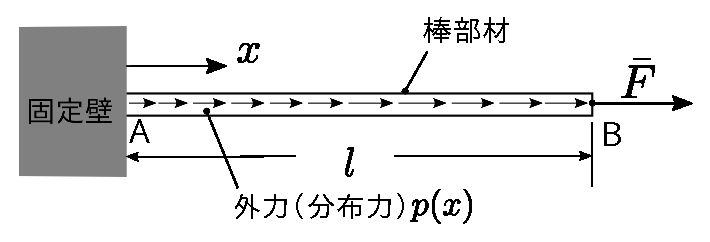
\includegraphics[width=0.4\linewidth]{fig1_1.eps} 
	\end{center}
	\caption{軸方向の外力$p(x)$と$\bar F$を受ける左端が固定支持された棒部材.} 
	\label{fig:fig1_1}
\end{figure}
部材の支持条件は図\ref{fig:fig1_1}に示したもの以外にも,例えば,
両端が固定された場合等が考えられるが,議論を具体的にするために,
以下では別途断りの無い限り, 図\ref{fig:fig1_1}の支持条件を対象として
一連の定式化方法(後述する弱形式、強形式)を示す.なお,一般の支持条件に
対しても同様な定式化は可能である.
\subsubsection{強形式と強解(新しい用語)}
以上で示したような,支配微分方程式(\ref{eqn:gveq})と境界条件(\ref{eqn:BC_u}),(\ref{eqn:BC_N})
による問題の定式化は{\bf 強形式(strong form)}と呼ばれ,その解$u(x)$のことを{\bf 強解(strong form solution)}と呼ぶ.
\subsection{弱形式}
\subsubsection{弱形式の導出}
$\xi (x)$を区間:$0\leq x \leq l$で定義され,$\xi(0)=0$を満たす任意の関数とする.
式(\ref{eqn:equiv_N})の両辺に$\xi (x)$を掛け,$x=0$から$x=l$の範囲で次のように
積分する.
\begin{equation}
	\int _0^l 
	\left(N'+p \right) \xi dx =0
	\label{eqn:int_gveq_xi}
\end{equation}
$N(x)$が軸力問題の解であれば,式(\ref{eqn:int_gveq_xi})は$\xi(x)$に依らず成立する.
式(\ref{eqn:int_gveq_xi})の左辺第一項を部分積分を用いて変形すると,
\begin{eqnarray}
	\int _0^l N'\xi dx &= & \left[ N\xi \right]_0^l -\int_0^l N \xi'dx  
	\label{eqn:int_by_part1}
	\\
	&= & \bar F \xi(l)  -\int_0^l N \xi'dx  
	\label{eqn:int_by_part2}
\end{eqnarray}
となる.ここで,式(\ref{eqn:int_by_part1})から式(\ref{eqn:int_by_part2})への変形には,
$\xi(0)=0$と$N(0)=0$であることを用いた.式(\ref{eqn:int_by_part2})を
式(\ref{eqn:int_gveq_xi})に代入して整理し,
\begin{equation}
	a(u,\xi) = \int_0^l N \xi'dx  
	= \int_0^l EA u' \xi'dx  
	\label{eqn:blinf_N}
\end{equation}
\begin{equation}
	b(\xi)= \bar F \xi (l) + 
	\int_0^l p\xi dx 
	\label{eqn:linf_N}
\end{equation}
と表すことにすれば,その結果は簡潔に次のように表すことができる.
\begin{equation}
	a(u,\xi)=b(\xi)
	\label{eqn:WF_N}
\end{equation}
式(\ref{eqn:WF_N})の関係は,$u(x)$が強解である限り$\xi(x)$に依らず成り立つことに注意する.
逆に,任意の$\xi(x)$について式(\ref{eqn:WF_N})を満足するような$u(x)$があったとし,
これを強解と区別して$\tilde u(x)$と書く.すなわち,$\tilde u(x)$は
\begin{equation}
	a(\tilde u,\xi)=b(\xi), \ \ (\forall \xi(x) \ {\rm s.t.} \ \xi(0)=0)
	\label{eqn:WF_N_tilde}
\end{equation}
の関係を満足するような関数であるとする.ここで,$\forall$は"for all (全ての,任意の)"と,
s.t.は"such that$\sim$($\sim$であるような)"と読む.従って,式(\ref{eqn:WF_N_tilde})は
$\xi(0)=0$であるような任意の$\xi(x)$について$a(\tilde u, \xi)=b(\xi)$が満たされる,
ということを述べたものである.式(\ref{eqn:WF_N_tilde})の関係を満たし,
$\tilde u(0)=0$となるような$\tilde u(x)$を求める問題を{\bf 弱形式(weak form)}と呼び,
その解である$\tilde u(x)$は{\bf 弱解}と呼ばれる.
\subsubsection{弱形式と強形式の等価性}
これまでの議論から,強形式の解$u$(強解)は必ず弱形式の解(弱解)になることは明らかである.
このことを図式的に書くと,
\begin{equation}
	強形式の解(強解) \ \Rightarrow \ 弱形式の解(弱解)
	\label{eqn:prop_s2w}
\end{equation}
となる.一方この逆,すなわち,弱解が同時に強形式の解となるか否かは自明で無い.
しかしながら,
\begin{equation}
	弱形式の解(弱解) \ \Rightarrow \ 強形式の解(強解)
	\label{eqn:prop_w2s}
\end{equation}
となることは以下のようにして示すことができる.\\

式(\ref{eqn:WF_N_tilde})の左辺を,部分積分により次のように変形する.
\begin{eqnarray}
	a(\tilde u, \xi) 
	&=& 
	\int_0^l EA\tilde u' \xi'dx \nonumber \\
	&=& 
	\left[ 
		EA \tilde u'\xi 
	\right]_0^l - \int_0^l (EA\tilde u')'\xi dx
	\nonumber \\
	&=&
	\left. EA \tilde u'\xi \right|_{x=l} - \int_0^l (EA\tilde u')'\xi dx
	\label{eqn:}
\end{eqnarray}
以上では,$\xi(0)=0$であることを用いた.一方,$\tilde u$が強解であるかどうか
この時点では不明であるため、$\tilde N = EA\tilde u'=\bar F$とすることはでき
ないことに注意が必要である.式(\ref{eqn:WF_N_tilde})に代入して整理すると,
\begin{equation}
	\int_0^l \left\{ (EA\tilde u')'+p \right\} \xi dx 
	+ \left\{ \bar F-EA\tilde u'(l) \right\}\xi(l)=0
	\label{eqn:w2s_proof}
\end{equation}
となる.$\xi(x)$は任意の関数でよいことから,適当な関数$\phi(x)$を用いて,
\begin{equation}
	\xi (x) =\left\{ (EA\tilde u')'+p \right\} \phi(x), \ \ (\phi(0)=0)
	\label{eqn:xi_special}
\end{equation}
としてもよい.さらに$\phi(x)$を
\begin{equation}
	\phi(x)= x(l-x)
	\label{eqn:}
\end{equation}
とすれば,$\xi(0)=\xi(l)=0$となるようにでき,これを踏まえて式(\ref{eqn:xi_special})の
$\xi(x)$を式(\ref{eqn:w2s_proof})に代入すると,
\begin{equation}
	\int_0^l \left\{ (EA\tilde u')'+p \right\}^2\phi dx =0
	\label{eqn:w2s_proof2}
\end{equation}
となることが分かる. 式(\ref{eqn:w2s_proof2})の被積分関数は全て正または零で,
$\phi(x)$は$0<x<l$で正である.従って,式(\ref{eqn:w2s_proof2})となるためには,
\begin{equation}
	(EA\tilde u')'+p =0
	\label{eqn:}
\end{equation}
でなければならない.このことを踏まえれば,式(\ref{eqn:w2s_proof})は,
任意の$\xi(l)$について
\begin{equation}
	\left\{ \bar F-EA\tilde u'(l)\right\}\xi(l) =0
	\label{eqn:}
\end{equation}
でなければならず,
\begin{equation}
	\tilde N =EA\tilde u' =\bar F
	\label{eqn:}
\end{equation}
が言える.以上のことから,式(\ref{eqn:WF_N_tilde})を満たすものの中で,
$\tilde u(0)=0$となるものは強形式の解であることがわかり,
\begin{equation}
	u=\tilde u
	\label{eqn:w2s}
\end{equation}
となることが結論される.すなわち,強形式と弱形式は同じ解を与え,この意味において
2つの問題の定式化は互いに等価なものということができる.
%%%%%%%%%%%%%%%%%%%%%%%%%%%%%%%%%
\subsection{仮想仕事式}
図\ref{fig:fig1_2}に示す2つの系を考える.これらの系では,部材に加えられた外力だけが互いに異なり,
支持条件と断面係数$E,A$は同じとする.そこで,系$i,\, (i=1,2)$に加えれた分布力を
$p_i(x)$,部材右端Bに作用する集中荷重を$\bar F_i$, その結果生じる変位と軸力をそれぞれ$u_i(x), N_i(x)$と表す.
\begin{figure}[h]
	\begin{center}
	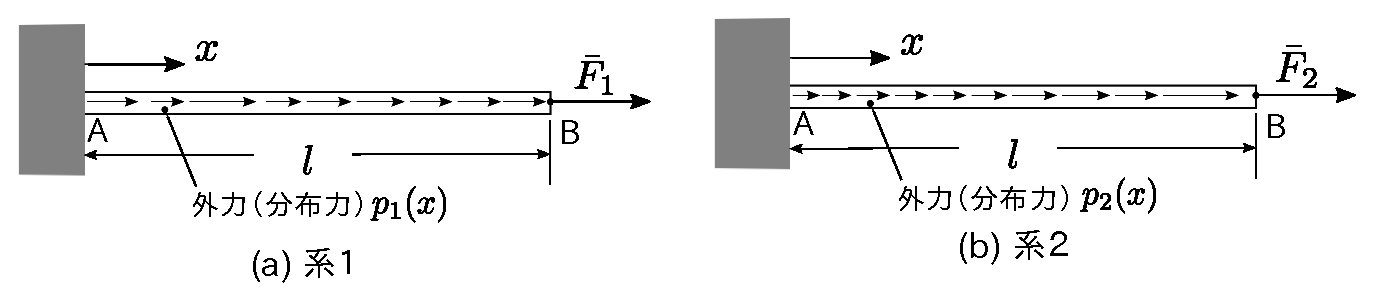
\includegraphics[width=0.8\linewidth]{fig1_2.eps} 
	\end{center}
	\caption{外力のみが異なる2つの系1と2.} 
	\label{fig:fig1_2}
\end{figure}
ここで式(\ref{eqn:WF_N})において,$u=u_1$, $\xi=u_2$とすれば,
\begin{equation}
	a(u_1,u_2)=\int_0^l N_1u_2'dx = \int_0^l\frac{N_1N_2}{EA}dx
	\label{eqn:vw_int}
\end{equation}
\begin{equation}
	b(u_2)=\bar F_1 u_2(l)+\int_0^l p_1 u_2dx
	\label{eqn:vw_ext}
\end{equation}
となり,これらの量が互いに等しいとの結果が得られる.
式(\ref{eqn:vw_int})と式(\ref{eqn:vw_ext})はともに,
力$\times$長さ,すなわち,仕事の次元を持つ量となっている.
前者は内力である$N_1$に, 後者は外力$\bar F_1$と$p_1(x)$に関する
ものであることから,これらの量をそれぞれ,内部仮想仕事,外部仮想仕事と呼ぶ.
"仮想"と呼ぶ理由は,力については系1,変位とひずみについては系2に関するもので,
両者の積が物理的に行われた仕事を指すものではないことによる.
系1と系2の間に成り立つ関係
\begin{equation}
	a(u_1,u_2)=b(u_2)
	\label{eqn:vw_eq}
\end{equation}
は,{\bf 仮想仕事式}と呼ばれる.
\subsection{力学的エネルギー保存則}
仮想仕事式(\ref{eqn:vw_eq})において$u_1=u_2$とする.すなわち,系1だけを考え,
弱形式(\ref{eqn:WF_N})において
\[
	u=u_1, \ \ \xi=u_1
\]
とした場合の仮想仕事式を考える.このとき,$a(u_1,u_2)$と$b(u_2)$は
それぞれ
\begin{equation}
	a(u_1,u_1)=\int_0^l N_1u_1'dx = \int_0^l\frac{N_1N_1}{EA}dx
	\label{eqn:w_int}
\end{equation}
\begin{equation}
	b(u_1)=\bar F_1 u_1(l)+\int_0^l p_1 u_1dx
	\label{eqn:w_ext}
\end{equation}
となる.いずれも
\[
	系1に作用する力 \times 系1に生じる変位 = 実際に行われた仕事
\]
であることから,
\begin{equation}
	a(u_1,u_1)=b(u_1)
	\label{eqn:energy_conservation}
\end{equation}
は,(仮想ではなく)実際に行われた外部仕事と内部仕事が等しいことを意味する.
通常,外力が過度に大きなものでない限り,外力を取り去れば部材は元の状態に
戻る.このことに加え,外力に起因して内力やひずみが発生するという見方をすれば,
外力による仕事として系に加えられたエネルギーは,内力やひずみのエネルギーとして
部材内部に蓄えられていると考えることができる.
仕事とエネルギーは同じ次元を持つことから,内力仕事を系内に蓄えられた
エネルギーの大きさとみなせば,式(\ref{eqn:energy_conservation})は,
系外から加えられたエネルギーと系内に蓄えられたエネルギーが等しいことを
示すと解釈できる.この意味で,式(\ref{eqn:energy_conservation})は
{\bf 力学的エネルギー保存則}を表している.
\subsection{単位荷重法}
仮想仕事式(\ref{eqn:vw_eq})における系1として,次のような特別な場合を考える.
\begin{equation}
	\bar F_1=0, \ \ p_1(x)=\delta(x-a), \ \ (0<a<l)
	\label{eqn:sys1}
\end{equation}
すなわち,図\ref{fig:fig1_3}に示すように,$x=a$に単位集中荷重だけが作用する場合を考える.
ここで,$\delta(x-a)$はディラクのデルタ関数を表し,
実数軸上全体で定義された任意の関数$f(x)$に対して,
次のような性質を持つ(証明は次節を参照).
\begin{equation}
	\int_{-\infty}^{+\infty} f(x) \delta(x)dx =f(0)
	\label{eqn:dlt_sampling}
\end{equation}
この性質を利用すれば,式(\ref{eqn:vw_ext})は次のようになる. 
\begin{equation}
	b(u_2)=\int_0^l \delta(x-a)u_2(x)dx= u_2(a)
	\label{eqn:vw_eq_dlt}
\end{equation}
そこで式(\ref{eqn:vw_eq_dlt})を仮想仕事式(\ref{eqn:vw_eq})に代入すれば,
\begin{equation}
	u_2(a)=\int_0^l \frac{N_1N_2}{EA}dx
	\label{eqn:u2_a}
\end{equation}
が得られる.これは,系1と系2のそれぞれにおける軸力$N_1$と$N_2$から,
$x=a$における系2の変位$u_2(a)$が求められることを意味する.
言い換えれば,系1を補助として用いれば,微分方程式を解くこと無く,
系2の変位が得られることを意味する.
そこで, 系1を補助系とし,系2を解くべき問題とする立場を明確にするために,
2つの系に関する諸量を,あらためて 
\begin{eqnarray}
	\left( u_1, N_1; \bar F_1, p_1 \right)& = &
		\left(\tilde u, \tilde N;\, \bar{\tilde{F}}=0, \tilde p= \delta(x-a) \right) 
	\label{eqn:aux}
	\\
	\left( u_2, N_2; \bar F_2, p_2 \right)& = &
		\left( u,  N;\, \bar F, p \right) 
	\label{eqn:prb}
\end{eqnarray}
と書くことにする.このとき,式(\ref{eqn:u2_a})は,
\begin{equation}
	u(a)=\int_0^l \frac{N \tilde N}{EA}dx
	\label{eqn:uload}
\end{equation}
と表され,この式(\ref{eqn:uload})を利用して変位を計算する解法を{\bf 単位荷重法}と呼ぶ.
\begin{figure}[h]
	\begin{center}
	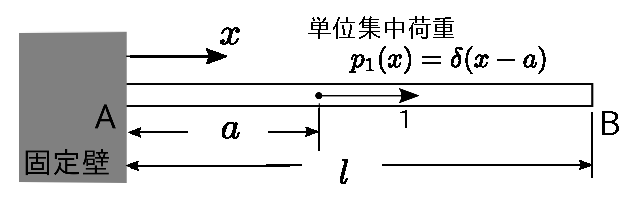
\includegraphics[width=0.4\linewidth]{fig1_3.eps} 
	\end{center}
	\caption{$x=a$に部材軸方向への単位集中荷重を受ける棒部材.} 
	\label{fig:fig1_3}
\end{figure}
\subsubsection{デルタ関数の性質}
式(\ref{eqn:dlt_sampling})が成り立つことの,簡易な証明は以下のようである.\\

デルタ関数を幅$2\varepsilon$の矩形関数:
\begin{equation}
	U(x;\varepsilon)=\left\{
	\begin{array}{cc}
		1/2\varepsilon & (|x|<\varepsilon) \\
		0 & (|x|>\varepsilon) \\
	\end{array}
	\right.
	\label{eqn:rec_fun}
\end{equation}
で近似する.これを,式(\ref{eqn:dlt_sampling})のデルタ関数の代わりに用いる.
さらに,$f(x)$の原始関数を$F(x)$と表せば,式(\ref{eqn:dlt_sampling})
左辺の積分は,次のように近似することができる.
\begin{equation}
	\int_{-\infty}^{+\infty} f(x) \delta(x)dx 
	\simeq 
	\int_{-\varepsilon}^{\varepsilon} f(x) \times \frac{1}{2\varepsilon}dx 
	=\frac{F(\varepsilon)-F(-\varepsilon)}{2\varepsilon}
	\label{eqn:dlt_apprx}
\end{equation}
この関係は$\varepsilon \rightarrow 0$において厳密に成り立つので,
式(\ref{eqn:dlt_apprx})の極限をとると,
\begin{equation}
	\int_{-\infty}^{+\infty} f(x) \delta(x)dx 
	=
	\lim_{\varepsilon \rightarrow 0} 
	\left\{
	\frac{F(\varepsilon)-F(-\varepsilon)}{2\varepsilon}
	\right\}
	=F'(0)=f(0)
	\label{eqn:}
\end{equation}
となり,式(\ref{eqn:dlt_sampling})が導かれる.
%
\newpage
\subsubsection{例題1}
図\ref{fig:fig1_4}-(a)に示す棒部材の点Bと点Cに発生する軸変位を,単位荷重法を用いて求めよ.
ただし,断面剛性$EA$は全断面で一定とする.
\begin{figure}[h]
	\begin{center}
	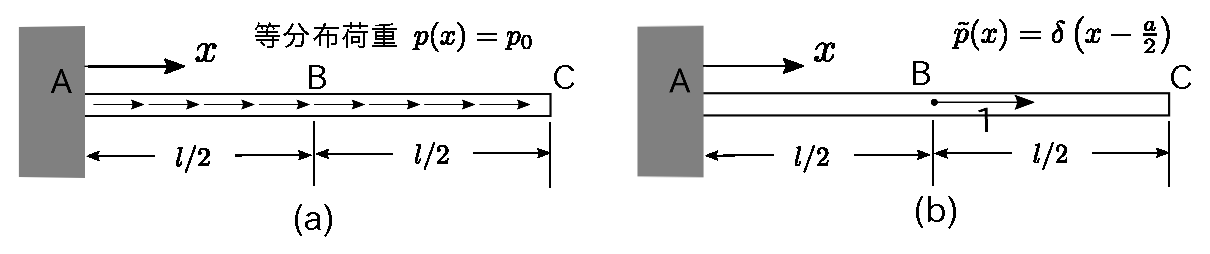
\includegraphics[width=0.4\linewidth]{fig1_4.eps} 
	\end{center}
	\caption{等分布荷重を受ける棒部材.}
	\label{fig:fig1_4}
\end{figure}
\paragraph{解答:}
式(\ref{eqn:u2_a})で表される単位荷重法を利用するためには,問題で与えられた系(図\ref{fig:fig1_4})に加え,
補助系を設定する必要がある.その際,点Bの変位を求めるためには点Bに(図\ref{fig:fig1_4_2}-(a)),
点Cの変位を求めるためには点Cに(図\ref{fig:fig1_4_2}-(c)),
それぞれ単位荷重を加えたものを各々の計算における補助系とすればよい.
式(\ref{eqn:u2_a})右辺の積分に含まれる$N$は,問題で与えられた系の軸力を,
$\tilde N$は補助系の軸力である.
従って,$N$と$\tilde N$を具体的に求て,式(\ref{eqn:u2_a})の積分を計算すれば,点Bや点Cの変位を得ることができる.
そこで,力の釣り合い条件から$N$を求めると図\ref{fig:fig1_4_1}のように,$\tilde N$を求めると,
図\ref{fig:fig1_4_2}の(b)および(d)のようになる.
\begin{figure}[h]
	\begin{center}
	\includegraphics[width=0.4\linewidth]{fig1_4_1.eps} 
	\end{center}
	\caption{軸力図.} 
	\label{fig:fig1_4_1}
\end{figure}
\begin{figure}[h]
	\begin{center}
	\includegraphics[width=0.8\linewidth]{fig1_4_2.eps} 
	\end{center}
	\caption{単位荷重法の適用において用いる補助系とその軸力図.} 
	\label{fig:fig1_4_2}
\end{figure}
従って,点Bの変位は$a=\frac{l}{2}$として,
\begin{equation}
	u\left(\frac{l}{2} \right)
	=
	\int _0^l \frac{N\tilde N}{EA}dx
	=
	\int _0^{l/2} \frac{p_0(l-x)\times 1}{EA}dx=\frac{3}{8}\frac{p_0l^2}{EA}
	\label{eqn:}
\end{equation}
と得られる.一方,点Cの変位は,$a=l$として次のように求められる.
\begin{equation}
	u(l)=\int_0^l\frac{p_0(l-x)\times 1}{EA}dx=\frac{p_0l^2}{2EA}
	\label{eqn:}
\end{equation}
\subsubsection{練習問題1}
図\ref{fig:fig1_5}に示す棒部材の,点Bの軸変位$u_B$と点Cの軸変位$u_C$を単位荷重法を
用いてそれぞれ求めよ.なお,断面剛性$EA$は全ての断面で一定とする.
\paragraph{解答:}
$u_B=\frac{\bar Fl}{2EA},\ u_C=\frac{\bar Fl}{EA}.$
\begin{figure}[h]
	\begin{center}
	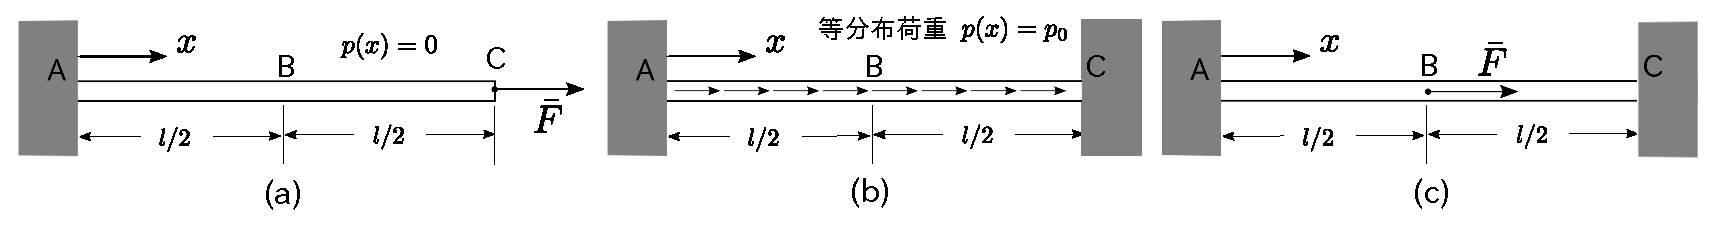
\includegraphics[width=0.4\linewidth]{fig1_5.eps} 
	\end{center}
	\caption{部材端部に集中荷重を受ける片端固定部材.} 
	\label{fig:fig1_5}
\end{figure}
\subsubsection{例題2}
図\ref{fig:fig1_6}に示す棒部材に作用する,支点反力の大きさと向きを答えよ.
\begin{figure}[h]
	\begin{center}
	\includegraphics[width=0.4\linewidth]{fig1_6.eps} 
	\end{center}
	\caption{等分布荷重を受ける両端固定部材.} 
	\label{fig:fig1_6}
\end{figure}
\paragraph{解答:}
支点反力の正方向を図\ref{fig:fig1_7}-(a)のように定めれば,与えられた系を
図\ref{fig:fig1_7}の(b)と(c)の重ね合わせで表現することができる.
ただし,系(c)で加えれれた力$H_C$は未知である.
ここで,系(b)の点Cにおける変位を$u_C^{(b)}$,
系(c)の点Cにおける変位を$u_C^{(c)}$とする.系(b)と系(c)の重ね合わせが
系(a)となるためには,
\[
	u_C^{(b)}+u_C^{(c)}=0
\]
でなければならない.$u_C^{(b)}$は例題1より,$u_C^{(c)}$は練習問題1で
$\bar{F}=H_C$と置くことにより,
\[
	u_C^{(b)}=\frac{p_0l^2}{2EA}
	, \ \ 	
	u_C^{(c)}=\frac{H_Cl}{EA}
\]
と得られ,$H_C=-\frac{p_0l}{2}$と決まる.その結果,部材全体の釣り合い条件より
\[
	H_A+H_C+p_0l=0 \ \Rightarrow \ H_A=\frac{p_0l}{2}
\]
となり,部材両端に作用する支点反力の大きさと向きが求められる.
支点反力が決定できれば,釣り合い条件から軸力分布も求めることができるようになる.

この問題で与えら得た系(両端固定部材)は不静定構造で,釣り合い条件だけから
断面力や反力を決定することが出来ない.しかしながら,上の解答にあるように,
与えられた系を2つの静定系に分割して変位の適合条件を課すことで支点反力を
求めることができる.その際,変位は部材中の一点(ここでは点C)で分かれば
よく,そのような場合,単位荷重法で効率よく必要な計算を行うことができる.
\begin{figure}[h]
	\begin{center}
	\includegraphics[width=0.4\linewidth]{fig1_7.eps} 
	\end{center}
	\caption{両端固定部材(a)の静定系(b)と(c)への分解.} 
	\label{fig:fig1_7}
\end{figure}
%----------------------------------
\end{document}
\subsubsection{練習問題2{\small (講義内課題$\Rightarrow$講義日中に解答をPDFファイルで提出)}}
図\ref{fig:fig1_8}の棒部材ACに作用する支点反力の大きさと向きを答えよ.また,軸力分布を求め,軸力図として示せ.
\begin{figure}[h]
	\begin{center}
	\includegraphics[width=0.4\linewidth]{fig1_8.eps} 
	\end{center}
	\caption{部材中央に集中荷重を受ける両端固定部材.} 
	\label{fig:fig1_8}
\end{figure}

